\documentclass[12pt,a4paper]{article}
\usepackage[utf8]{inputenc}
\usepackage[francais]{babel}
\usepackage[T1]{fontenc}
\usepackage{amsmath}
\usepackage{amsfonts}
\usepackage{amssymb}
\usepackage{graphicx}
\usepackage{kpfonts}

\usepackage{siunitx}

\usepackage{pgfplots}

\author{Mathieu Leocmach}
\begin{document}

\section{Gel en contact avec le fond}

\begin{figure}
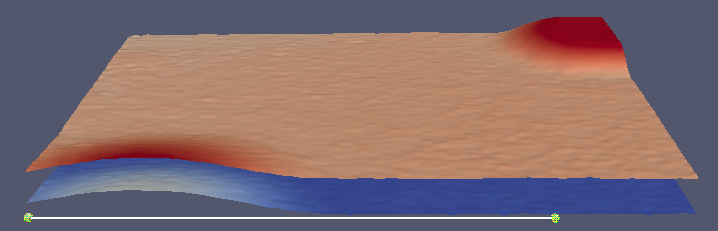
\includegraphics[width=\textwidth]{plots_0117.png}
\caption{Un exemple de cloque en train de croitre (premier plan). Au fond : une cloque qui a touché une paroi. La barre fait \SI{1}{\milli\metre}.}
\end{figure}

On considère une cloque de diamètre $\lambda$ dont le contour touche la paroi inférieure et dont le sommet s'est élevé d'une hauteur $A(t)$ à l'instant $t$. On considère que $A \ll \lambda$, donc l'aire reste $\lambda^2$.

En généralisant Vella PRL 2009, on considère $\sigma$ une contrainte s'exerçant uniformément sur la cloque suivant $z$. Minimiser l'énergie revient à minimiser la fonctionnelle
\begin{equation}
\mathcal{F} = \int_0^{\lambda/2}\left\lbrace\frac{1}{2} B \theta_s^2 + \sigma z - \Sigma \left[1-\frac{\Delta \lambda}{\lambda} - \cos\theta\right] \right\rbrace ds
\end{equation}
avec $s$ l'abcisse curviligne, $\theta(s)$ l'angle avec l'horizontale, $B$ le module de flexion $B \sim E h^3 /12 / (1-\nu^2) \sim G' h^3/10$.

Une longueur caractéristique apparaît :
\begin{equation}
\lambda^* = \left(\frac{B}{\sigma}\right)^\frac{1}{3}
\label{eq:lstar}
\end{equation}
au dessus de laquelle $\sigma$ est capable d'écraser la cloque.

\paragraph*{Si $\sigma = \Delta\rho g h$}, c'est une longueur élastogravitaire

Dans notre cas $\Delta\rho\simeq 10\%w = \SI{100}{\kilo\gram\per\metre^3}$, d'où
\begin{equation}
\lambda^* \sim \left(\frac{\num{6e-12}}{100\times 10 \times \num{50e-6}}\right)^\frac{1}{3} \sim \SI{0.4}{\milli\metre}
\end{equation}
Donc la gravité pourrait influer, ce qui est infirmé par un échantillon vertical plissant.

\paragraph*{Si $\sigma$ est une pression de Darcy $P$} telle que 
\begin{equation}
\vec{v} = - \frac{\ell_p^2}{\eta}  \vec{\nabla} P
\label{eq:Darcy}
\end{equation}
avec $v$ le flux volumique à travers la surface, c'est-à-dire la vitesse de déplacement du film, $\ell_p$ la taille des pores, $\eta$ la viscosité du solvant et $\vec{\nabla} P \sim -P/h$. Alors,
\begin{equation}
\lambda^* \sim \left(\frac{B \ell_p^2}{\eta v h}\right)^\frac{1}{3}
\end{equation}

On a mesuré $v\simeq \SI{0.2}{\micro\metre\per\second}$, et $\ell_p=\SI{4}{\micro\metre}$, ce qui donne 
\begin{equation}
\lambda^* \sim \left(\frac{\num{6e-12} (\num{4e-6})^2}{10^{-3} \times \num{0.2e-6} \times \num{50e-6}}\right)^\frac{1}{3} \simeq \SI{2}{\milli\metre}
\end{equation}

D'après Kolinski PRL 2009, aux faibles déformations la longueur d'onde effective est $\lambda \sim \epsilon^{1/7} \lambda^*$ avec $\epsilon$ le gain relatif de longueur du film. L'amplitude, elle, s'écrit $A \sim \epsilon^{4/7} \lambda^*$. On remarque que la base de la cloque n'évolue plus après que son sommet ait touché le plafond, c'est à dire que la longueur d'onde est sélectionnée quand $A=e-h\equiv H$.

Ca nous donne $\lambda \sim \epsilon^{-3/7} H$. On retrouve ainsi la proportionalité entre la longueur d'onde et l'épaisseur de la cellule.
\begin{equation}
\epsilon \sim \left(\frac{\lambda}{e}\frac{e}{H}\right)^{-4/3} \simeq \left(15\times 2\right)^{-7/3} \simeq \num{3e-4}
\end{equation}
Ce qui correspond tout à fait aux mesures expérimentales de l'excès d'aire au moment où les cloques se forment.

On avait remarqué que lorsque des cloques se forment, la longueur d'onde est environ moitié plus petite que lorsque des plis se forment de façon homogène. Si les plis se forment bien à $\lambda^*$ (voir plus bas), les cloques ont une taille de $\epsilon^{1/7} \lambda^*$, or avec la valeur ci-dessus, on trouve $\epsilon^{1/7}\simeq 0.3$.

\pagebreak

\section{Gel au milieu de la cellule}

\begin{figure}
\begin{tikzpicture}
\begin{axis}[
	width=\textwidth, height=0.25\textwidth, scale only axis,
	domain=0:360, no markers, ymin=-4, ymax=4,xmin=0,xmax=360,
	axis y line=none, xtick=\empty,
	]
\addplot+[orange]{sin(x)+0.5};
\addplot+[orange]{sin(x)-0.5};
\addplot+[dashed, black]{0.5};
\addplot+[dashed, black]{-0.5};
\draw[<->] (axis cs:180,0.5) -- (axis cs:180,4) node[midway, left] {$H$}; 
\draw[<->] (axis cs:30,-0.5) -- (axis cs:30,-4) node[midway, left] {$H$};
\node[below] at (axis cs:90,0.5) (pb1) {$P_1$};
\node[above] at (axis cs:90,1.5) (ph2) {$P_2$};
\node[above] at (axis cs:270,-0.5) (ph1) {$P_1$};
\node[below] at (axis cs:270,-1.5) (pb2) {$P_2$};
\draw[thick, ->] (ph2) -- (pb1);
\draw[thick, ->] (pb2) -- (pb1);
\end{axis}
\end{tikzpicture}
\end{figure}

On considère maintenant une couche de gel d'épaisseur $h$ centrée à mi-hauteur de la cellule. La distance moyenne entre une surface du film et la paroi la plus proche est notée $H$. On considère une perturbation sinusoïdale.

Par symmétrie, la différence de pression à travers le poreux est la même qu'entre un minimum et un maximum d'altitude du film. Sur cette demi-longueur d'onde, on suppose un écoulement de Poiseuille dans la couche d'eau d'épaisseur $H$. 

\begin{equation}
\Delta P \sim 12\eta\frac{\lambda}{H^2} u
\end{equation}
où $u$ est la valeur moyenne de la vitesse suivant $x$. Dans l'hypothèse de lubrification, la vitesse suivant $z$ est $v\sim \frac{H}{\lambda} u$, donc
\begin{equation}
\Delta P \sim 12\eta\frac{\lambda^2}{H^3} v
\end{equation}

En injectant ce résultat dans l'équation (\ref{eq:lstar}), on obtient la longueur au delà de laquelle l'écoulement de Poiseuille interdit la déformation :
\begin{equation}
\lambda^*_\text{Poiseuille} \sim \left(\frac{B H^3}{12\eta v}\right)^\frac{1}{5}
\end{equation}

En prenant $H=\SI{30}{\micro\metre}$, on obtient
\begin{equation}
\lambda^*_\text{Poiseuille} \sim \left(\frac{\num{6e-12} (\num{30e-6})^3}{12 \times
10^{-3} \times \num{0.2e-6}}\right)^\frac{1}{5} \simeq \SI{2}{\milli\metre}
\end{equation}
Ce qui est comparable à la longueur d'onde de Darcy pour notre expérience typique (caséine 4\%, GDL 4\% dans l'eau pure à \SI{21}{\celsius}).

Pour une longueur d'onde donnée, les vitesses de croissances respectives sont
\begin{align}
v_\text{Darcy} &\sim \frac{B \ell_p^2}{\eta h \lambda^3}\\
v_\text{Poiseuille} &\sim \frac{B H^3}{12\eta \lambda^5}
\end{align}
D'où leur rapport
\begin{equation}
\frac{v_\text{Darcy}}{v_\text{Poiseuille}} \sim \frac{\ell_p^2\lambda^2}{hH^3}
\end{equation}

On note que ce rapport est indépendant des propriétés viscoélastiques du système ($B$ et $\eta$) et est donc pûrement géométrique. La croissance des modes de Darcy est plus rapide quand les pores sont gros, la longueur d'onde importante et le système fin.

Pour les deux concentrations où on connaît la taille des pores (4\% de caséine à \SI{21}{\celsius}, on suppose $h=\SI{40}{\micro\metre}$ et $H=\SI{30}{\micro\metre}$ dans les deux cas) on a les rapports de vitesses :
\begin{itemize} 
\item 4\% de GDL, dans l'eau pure : 37
\item 8\% de GDL, dans 60\% de glycérol : 75
\end{itemize}
Le mode de Darcy semble donc être cinétiquement favorisé dans (la pluspart de) nos expériences.


\end{document}